% !TEX root = ../thesis.tex

\vspace{-10pt}

\section{Formative User Evaluations}

\vspace{-10pt}

Lyra was designed to support both expressive and \emph{accessible} visualization
design: users should not require coding expertise to be able to construct custom
visualizations. To evaluate Lyra's accessibility, we conducted first-use studies
with 15 representative users including 6 data analysts / visualization
designers, 5 data journalists, and 4 graduate students in data visualization. On
10-point scales, the median self-reported visualization design expertise was 7,
while programming expertise range between 2--8. These users all use
visualization as a communicative medium but their processes for creating them
vary. The visualization designers and grad students were more technically
proficient and typically use D3, whereas the data journalists rely on chart
typologies (Microsoft Excel) or grammar-based systems (Tableau) that do not
require programming. Some journalists also reported eschewing visualization
systems in favor of drawing programs such as Adobe Illustrator.

\vspace{-10pt}

\subsection{Methods}

\vspace{-7pt}

We began each study with a 10 minute tutorial. We then asked participants to
design three graphics: a bar chart of medal count by country at the 2012
Olympics (T1), a grouped or stacked bar chart of medal counts by medal type and
country (T2), and a trellis plot of barley yields (T3,
Fig.~\ref{fig:lyra:trellis}). These tasks were designed to ensure participants
interacted with all aspects of Lyra. Each task was more difficult than the
previous, intending to first familiarize participants with the Lyra design
process, and then challenge them. Participants were encouraged to think-aloud
and were de-briefed at the end. Sessions lasted approximately 45 minutes, after
which we administered a post-study survey.

\begin{figure}[b!]
  \centering
  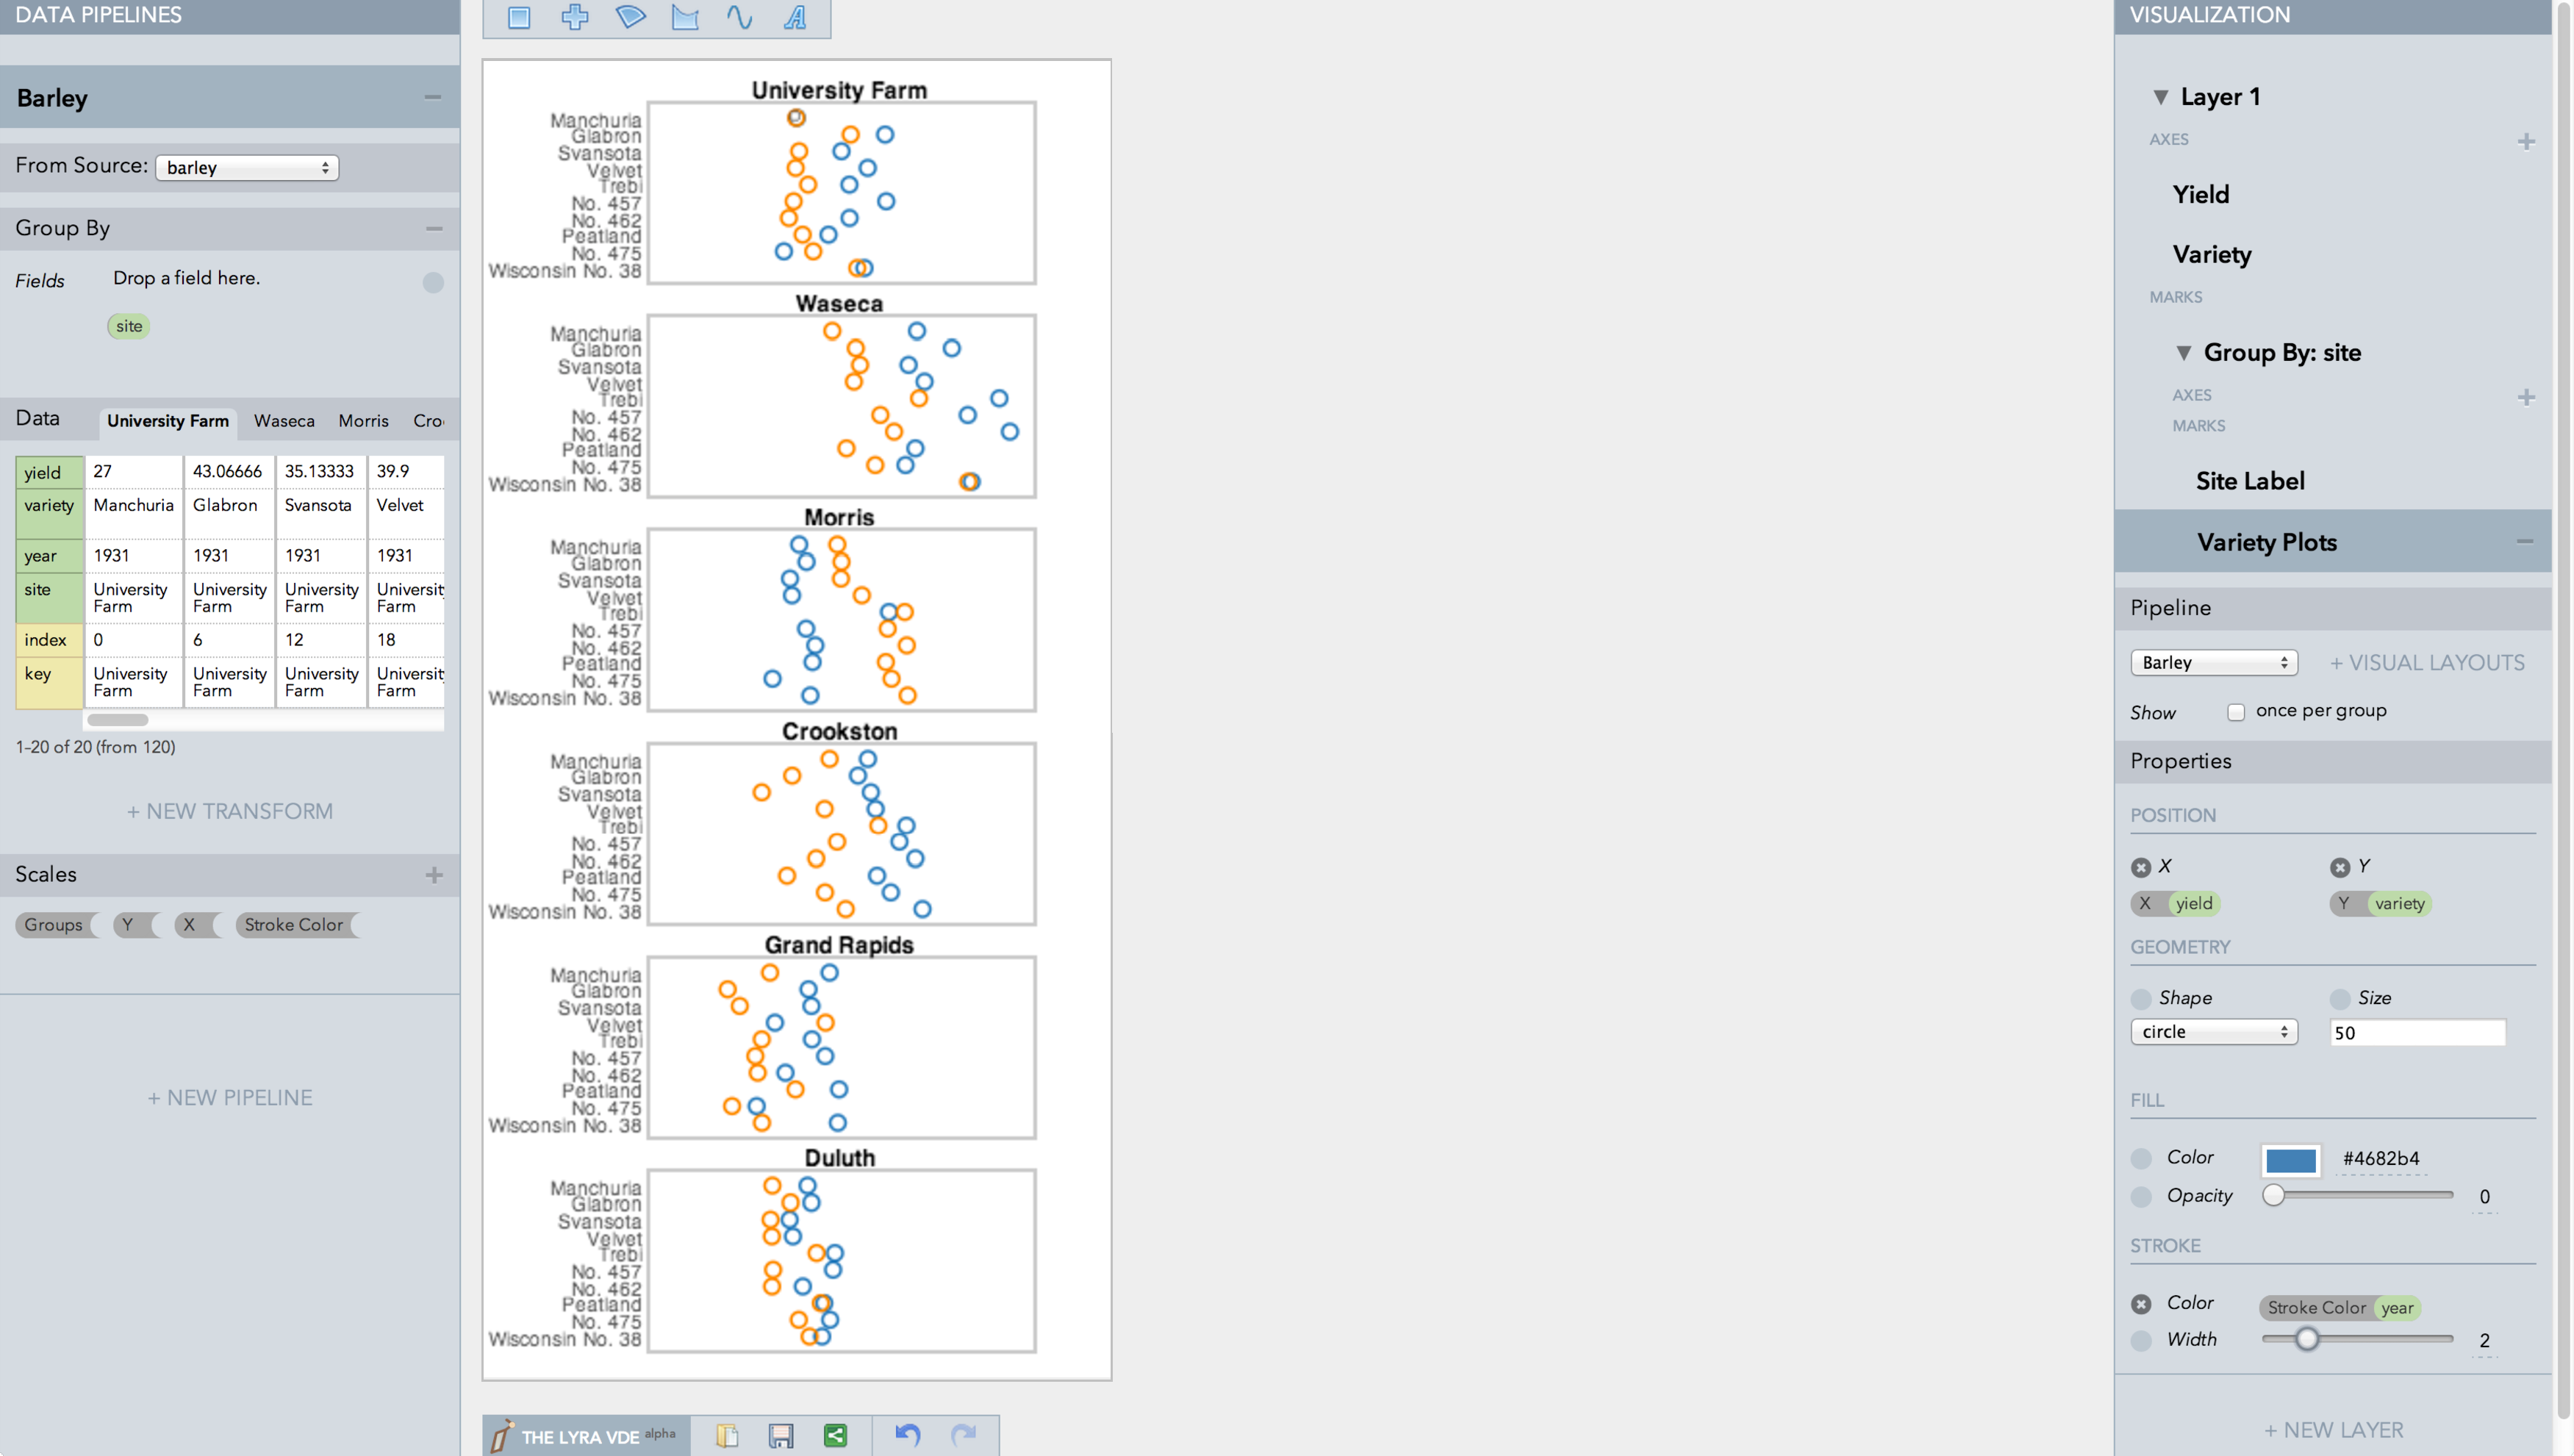
\includegraphics[width=1\columnwidth]{barley}
  \caption{Study participants recreated the barley yields Trellis
  display~\cite{becker:trellis}.}
  \label{fig:lyra:trellis}
\end{figure}

\vspace{-10pt}

\subsection{Successes}

\vspace{-7pt}

Users quickly learned Lyra's interaction model and all users, regardless of
their technical expertise, successfully completed all three tasks with minimal
guidance (100\% task completion rate). Users completed the first two tasks in
just a few minutes, the more complex third task took longer (T1: median time =
1:33, inter-quartile range (IQR) = 0:51; T2: median = 2:43, IQR = 2:57; T3:
median = 10:24, IQR = 4:00). In a post- study survey, users rated Lyra's
interface highly: drop zones felt natural to use ($\mu$ = 4.4, $\sigma$ = 0.57
on a 5-point Likert scale), connectors helped to relatively position marks
($\mu$ = 4.3, $\sigma$ = 0.49), and a pipeline's data table helped evaluate
context ($\mu$ = 4.4, $\sigma$ = 0.51). Handles were found useful for resizing
and positioning ($\mu$ = 3.8, $\sigma$ = 0.45) but users noted that the
properties they control are typically mapped to data. When asked to recount
their experience, users described drop zones as \emph{``natural''} and
\emph{``intuitive.''} One user stated, ``\emph{it's like \emph{literally} saying
`put that there.'}'' Others drew comparisons to Tableau's shelves:
\emph{``[shelves] don't always behave like I expect them to but [drop zones]
make me feel more in control.''} One participant ended his session by saying
that \emph{``there's a real joy in using Lyra.''}

Two journalists who participated lead data visualization teams in their
organizations. They appreciated that Lyra took cues from familiar drawing tools.
They welcomed Lyra's image export options, particularly SVG export, as the
visualizations they produce are often reutilized in print media. One suggested
that Lyra could be a powerful training tool that could help familiarize his team
with the process of designing visualizations from the ground-up.

\begin{figure}[b!]
\centering
  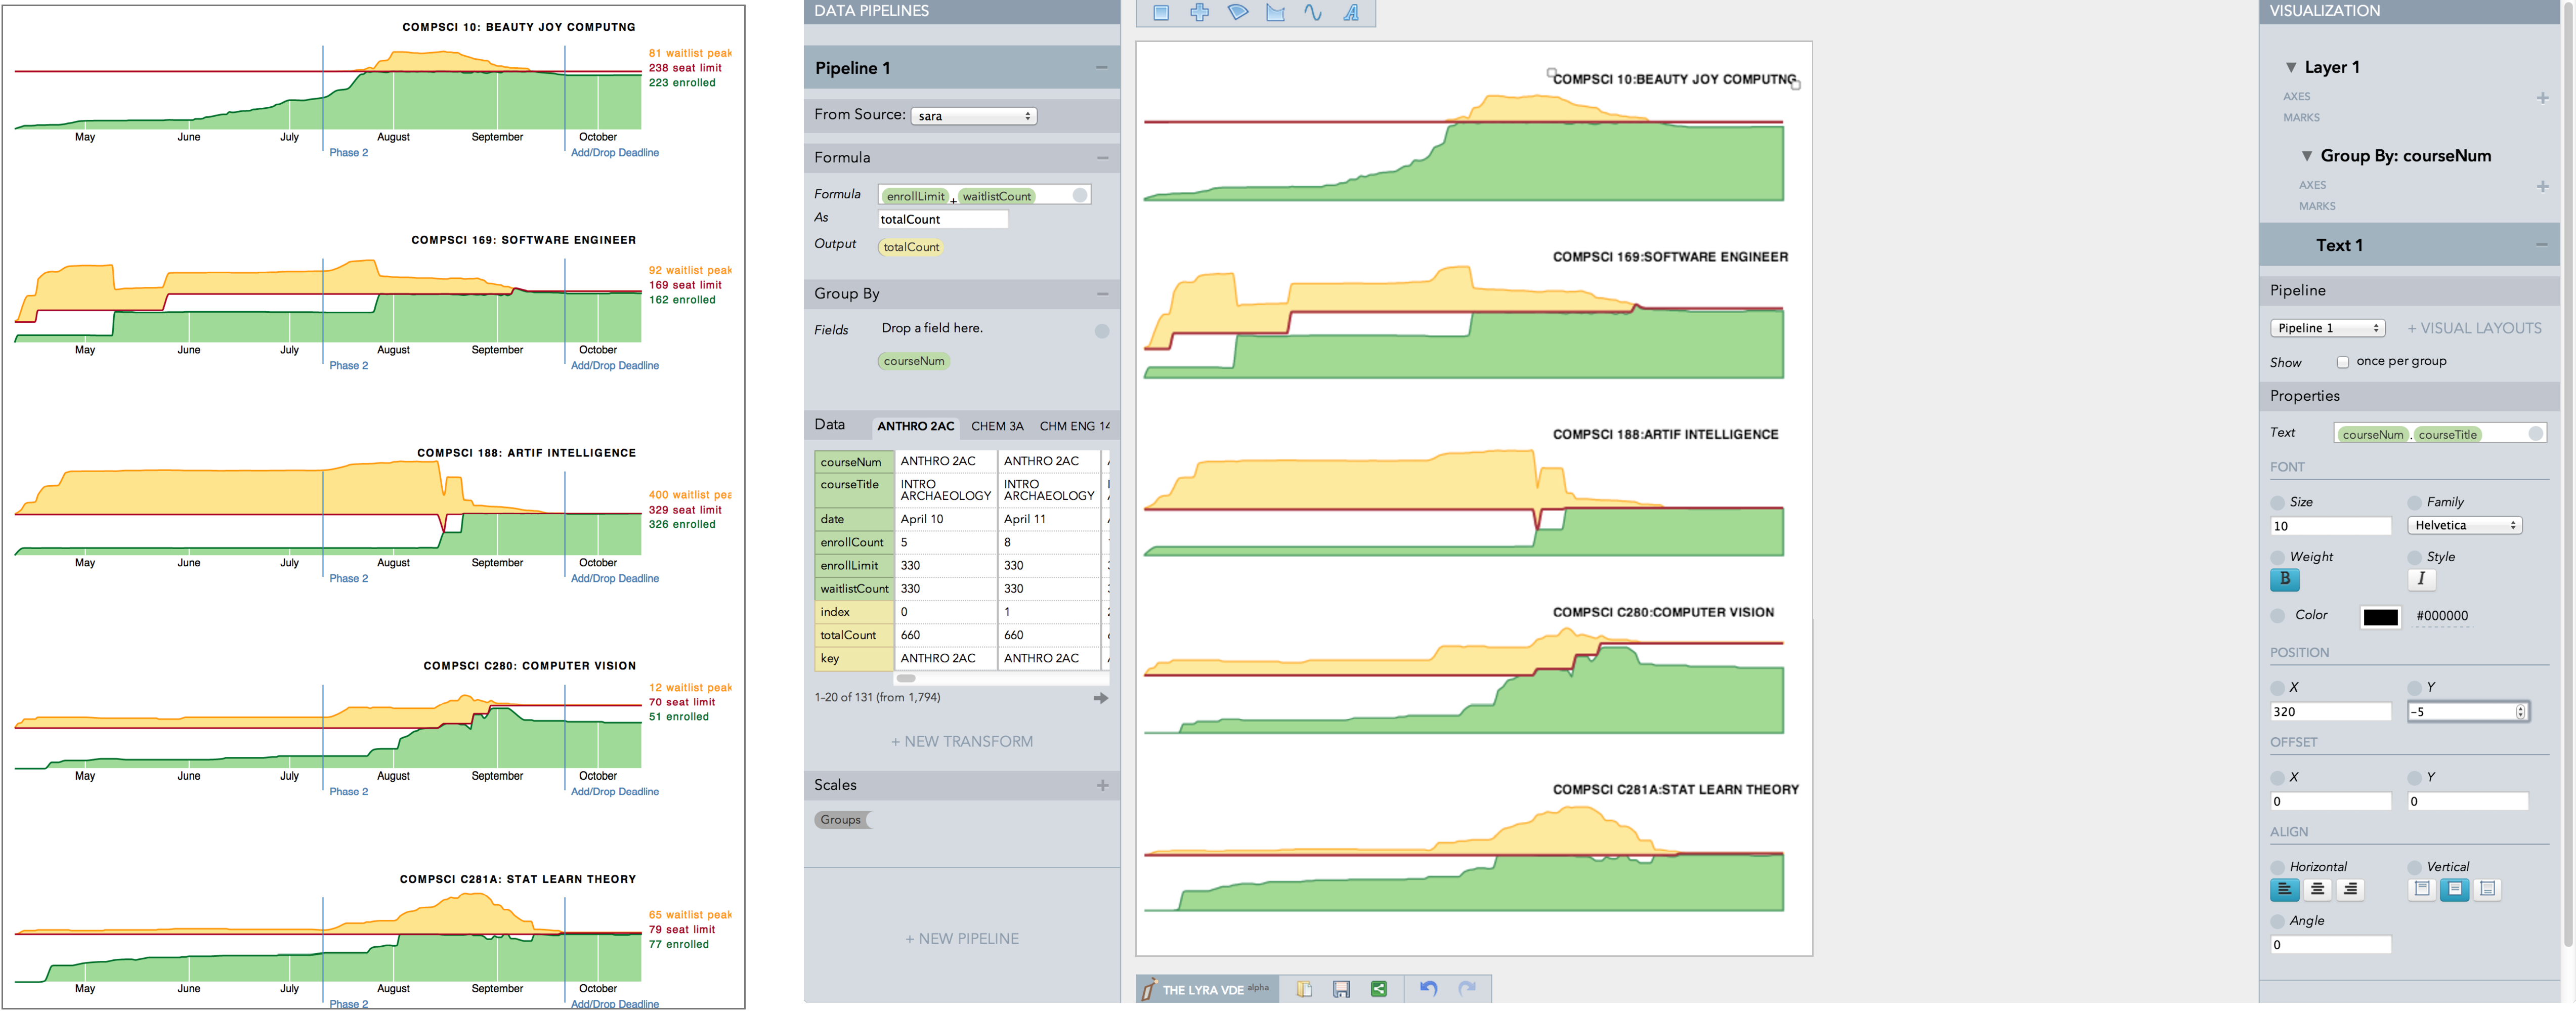
\includegraphics[width=\columnwidth]{sara}
  \caption{A study participant approximately recreated a D3 visualization (left,
  requiring 4-6 hours) in Lyra (right, requiring only 10 minutes).}
  \label{fig:lyra:sara_waitlists}
\end{figure}

Users familiar with lower-level tools such as D3 found Lyra useful for rapidly
prototyping and iterating on their design. For example, one user (self-rated
expertise with D3 as 6.5/10) used Lyra with her own data. By her estimate, she
had previously spent between 4--6 hours repurposing an existing D3 example to
create a custom visualization. She was able to create a close approximation in
Lyra, shown in \cref{fig:lyra:sara_waitlists}, in only 10 minutes.

\subsection{Shortcomings}

We also observed that Lyra posed certain challenges for our participants.
Although users found drop zones natural and intuitive, they noted problems with
the current implementation. First, when users missed a drop zone by a few
pixels, they expected Lyra to infer their intent. Second, when users
successfully dropped a field, they would lose track of the currently selected
mark if it was repositioned. A third shortcoming was Lyra's lack of support for
undo, which led users to become more hesitant to freely explore. Undo support
has since been added to Lyra, and we plan to address the remaining issues in
future versions. For example, a Voronoi diagram could be used to find the
nearest drop zone~\cite{grossman:bubble}, and staggered animated transitions
could help users better track changes~\cite{heer:animated} to marks.

Finally, several users mentioned that learning from and repurposing existing
visualizations is an important part of their design process. They found the
blank canvas to be an intimidating starting point. We anticipate that
providing a gallery of examples (including those in this paper) that users can
import, reuse and modify would mitigate this issue.
